\documentclass[12pt,fleqn]{article}\usepackage{../../common}
\begin{document}
Ders 29

Nihayet en son ayrıştırma (decomposition) konusuna geldik, bu teknik Eşsiz Değer
Ayrıştırma (Singular Value Decomposition -SVD-) tekniğidir. Ayrıştırma şu halde
olacak

$$ A = U \Sigma V^T $$

Sağ tarafta ayrışma sonrası bir dikgen (orthogonal) matris, bir köşegen
(diagonal) matris, ve tekrar bir dikgen matris olacak. Yani bildiğimiz,
sevdiğimiz matris formları ayrışma sonrası parçalar olarak elimize
geçecekler. İlginç olan iki tane dikgen matris elde etmemiz. Ayrıca $A$
her türden, her boyuttan bir matris olabilir (illa karesel olması gerekmez
mesela).

SVD bu dersin pek çok kavramını da bir araya getirir. Mesela simetrik
pozitif kesin matrisler. Hatırlarsak bu matrisler simetrik olduğu için
özvektörleri dikgen idi. Yani normalde şu haldeki bir ayrışma

$$ A = S \Lambda S ^{-1}   $$

Su halde gorulebiliyordu

$$ A = Q \Lambda Q ^{T}   $$

Yani $S$, dikgen vektörlü $Q$ oluyordu, pozitif kesinlik sayesinde de
normal bir $\Lambda$, içinde sadece pozitif değerler taşıyan bir  $\Lambda$
oluyordu. 

Özetle, eğer $A$ simetrik pozitif kesin ise onun SVD'si $Q \Lambda Q ^{T}$
olacaktır. Bu durumda tek $Q$ matrisi yeterli, diğer durumlarda $U,V$ gibi
iki farklı matris lazım. Ayrıca şunu da vurgulayalım: SVD için dikgenlik
aradığımız önemli bir şart, ``dikgen çarpı köşegen çarpı dikgen''
şeklinde bir form istiyorum özellikle. 

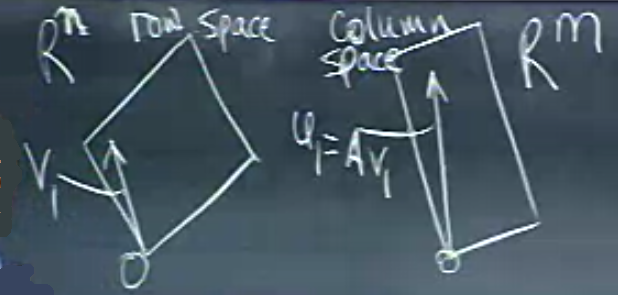
\includegraphics[height=4cm]{29_1.png}

SVD'den beklediğimiz işlemi yukarıdaki resim üzerinden anlamaya
çalışalım. Soldaki düzlem satır uzayı (row space), sağdaki kolon uzayı
(column space). Bir matrisi temsil eden satırlar ve kolonlar bu uzayların
içinde. Şimdi eğer $U \Sigma V^T$ formunu düşünürsek, öyle bir köşegen
matris arıyorum ki satır uzayındaki dikgen bazı (basis) uzayındaki bir
dikgen baza transform etmeli. Bu hakikaten özel bir matris olmalı.

Soru: satır uzayının dikgen bazı var mıdır? Tabii ki vardır,
Gram-Schmidt tekniğinde gördük, herhangi bir bazın dikgen bazını
alabiliriz. Dikgen baz hesabı özgün değildir, aynı bazdan pek çok
dikgen baz çıkartılabilir, ve satır uzayındaki ``herhangi'' bir
dikgen bazı alıp kolon uzayına transform edersem onun illa dikgen
kalacağı garanti değildir. Yani transform edildikten sonra da dikgen
kalacak özel bir dikgen baz arıyorum. Yapmaya çalıştığım çarpım her
vektörü gösterecek şekilde nasıldır?

$$ 
A \left[\begin{array}{rrrr}
& & & \\ v_1 & v_2 & ... & v_r 
\\ & & & 
\end{array}\right] = 
\left[\begin{array}{rrrr}
& & & \\ u_1 & u_2& ... & u_r \\ 
& & & 
\end{array}\right] 
\left[\begin{array}{rrrr}
\sigma_1 & & & \\  
& \sigma_2&  & \\ 
& & \ddots & \\ 
& & & \sigma_r
\end{array}\right] 
$$

Yani $Av_1$ çarpımı bana $u_1 \sigma_1$'i vermeli. Matris olarak yukarıdaki 

$$ AV = U\Sigma $$

Hatta dikgenlikten daha ileride birimdikliği (orthonormal) hesaplamak daha
da iyi.

Örnek 

$$ 
A = 
\left[\begin{array}{rr}
4 & 4 \\ -3 & 3
\end{array}\right]
 $$

$A$ tersine çevirilebilir (invertible) o zaman kertesi (rank)
2. Aradıklarım 

$$ v_1,v_2 \  \mathbb{R}^2 \textit{ satır uzayında }  $$

$$ u_1,u_2 \  \mathbb{R}^2 \textit{ kolon uzayında }  $$

$$ \sigma_1 > 0, \sigma_2 > 0 $$

Sıfır uzayı (nullspace) burada problem değil. Zorluklar neler? Matris
simetrik olmayabilir, o zaman özvektörleri kullanamam, çünkü onlar
dikgen değildir.

$$ A = U \Sigma V^{-1} $$

$V^{-1}$'yi başka nasıl yazabilirim? $V$ kare, dikgen olacağına göre,
$V^{-1} = V^{T}$. O zaman 

$$ A = U \Sigma V^{T} $$

Şimdi hesabı düşünmeye başlayalım. İki tane ayrı dikgen matris bulmam
lazım, ama bunların ikisini de aynı anda bulmak istemiyorum. Bir fikir:
öyle bir numara yapayım ki $U$ yokolsun her şey $V$ üzerinden temsil
edilsin. 

Alttaki ifade ne zaman elimizde genel dikdörtgensel (kare olmayan) bir
matris varsa karşımıza çıkan bir ifade, $A^TA$. Bu matris kare, pozitif
kesin, yani güzel özellikleri var. O zaman üstteki formülü $A^T$ ile soldan
çarpacağız,

$$ A^T = V \Sigma^T U^{T}  $$

olduğuna göre,

$$ A^TA = V \Sigma^T U^{T}  U \Sigma V^{T}  $$

$U^TU = I$ olduğuna göre

$$ A^TA = V \Sigma^T \Sigma V^{T}  $$

Kolaylaştırmalar bitmedi. $\Sigma$ köşegen olduğuna göre, $\Sigma^T\Sigma$
köşegendeki değerlerin karesinden ibarettir. 

$$ = V 
\left[\begin{array}{rrrr}
\sigma_1^2 &&& \\
 & \sigma_2^2 &  & \\
&& \ddots & \\
&&& \sigma_r^2 
\end{array}\right] 
V^T
  $$

İşte, $U$'lar yokoldu. Bu son ulaştığımız formda $V$'ler nedir?
Özvektörlerdir! Problem mükemmel bir özdeğer / özvektör problemine
dönüştü, yani $Q\Lambda Q$ haline geldi. Bu kolaylığa, sonuca $A$ yerine $A^TA$'yi
kullanmak sayesinde eriştik.

Pekala bu şekilde $V$'leri elde ediyoruz, ama $U$'yu nasıl elde edeceğiz?
Onu geçici bir süre için yokettik, ama $U$ hala hesaplamamız gereken bir
büyüklük, vektörler. Onun da çaresi var, $A^T$ ile soldan çarpmak yerine ana
formülü $A^T$ ile sağdan çarparsak, bu sefer $V$'ler yokolur, ve yine
benzer özdeğer / özvektör hesabına geliriz, ama bu sefer $U$ hesaplarız.

$$ AA^T = U\Sigma V^TV\Sigma^TU^T $$

$$  = U\Sigma \Sigma^TU^T $$

Örnek için tüm bu hesapları yapalım. 

$$ 
A^TA = 
\left[\begin{array}{rr}
4 & -3 \\ 4 & 3
\end{array}\right]
\left[\begin{array}{rr}
4 & 4 \\ -3 & 3
\end{array}\right] = 
\left[\begin{array}{cc}
25 & 7 \\ 7 & 25
\end{array}\right]
$$

Özvektörler

$$ 
\left[\begin{array}{r}
1 \\ 1
\end{array}\right],
\left[\begin{array}{r}
-1 \\ 1
\end{array}\right]
 $$

Özdeğerler

$\lambda_1=32, \lambda_2=18$. 

Özvektörleri normalize etmeli

$$ 
\left[\begin{array}{r}
1 / \sqrt{ 2} \\ 1/ \sqrt{ 2}
\end{array}\right],
\left[\begin{array}{r}
-1/ \sqrt{ 2} \\ 1/ \sqrt{ 2}
\end{array}\right]
 $$

o zaman 

$$ 
\underbrace{
\left[\begin{array}{rr}
4 & 4 \\ -3 & 3
\end{array}\right] 
}_{A}
=
\underbrace{
\left[\begin{array}{rr}
 &  \\  & 
\end{array}\right]
}_{U}
\underbrace{
\left[\begin{array}{rr}
\sqrt{ 32} &  \\  & \sqrt{ 18}
\end{array}\right]
}_{\Sigma}
\underbrace{
\left[\begin{array}{rr}
1/\sqrt{ 2} & 1/\sqrt{ 2} \\ -1/\sqrt{ 2} & 1/\sqrt{ 2}
\end{array}\right]
}_{V^T}
 $$

Şimdi $U$'nun sırası geldi. Onun için $AA^T$ lazım. 

$$ A^TA = 
\left[\begin{array}{rr}
4 & 4 \\ -3 & 3
\end{array}\right] 
\left[\begin{array}{rr}
4 & -3 \\ 4 & 3
\end{array}\right] =
\left[\begin{array}{rr}
32 & 0 \\ 0 & 18
\end{array}\right]
 $$

Raslantı oldu yukarıdaki çarpım köşegen çıktı, iyi oldu tabii, çünkü bu tür
matrislerin özvektörlerini, özdeğerlerini hesaplamak çok
kolaydır. Özvektörler, 

$$ 
\left[\begin{array}{r}
1 \\ 0
\end{array}\right],
\left[\begin{array}{r}
0 \\ 1
\end{array}\right]
 $$

Özdeğerler $\lambda_1 = 32, \lambda_2 = 18$

İlginci ki yine aynı özdeğerleri elde ettim, ama şaşırmamak lazım, çünkü
mesela bir $AB$ çarpımının özdeğerleri $BA$ ile aynıdır. 

Neyse $U$'yu bulduk, yerine koyalım, 

$$ 
\underbrace{
\left[\begin{array}{rr}
4 & 4 \\ -3 & 3
\end{array}\right] 
}_{A}
=
\underbrace{
\left[\begin{array}{rr}
1 & 0 \\ 0 & 1 
\end{array}\right]
}_{U}
\underbrace{
\left[\begin{array}{rr}
\sqrt{ 32} & 0 \\ 0 & \sqrt{ 18}
\end{array}\right]
}_{\Sigma}
\underbrace{
\left[\begin{array}{rr}
1/\sqrt{ 2} & 1/\sqrt{ 2} \\ -1/\sqrt{ 2} & 1/\sqrt{ 2}
\end{array}\right]
}_{V^T}
 $$

Örnek 

Bu sefer $A$ eşsiz (singular) olsun, yani kertesi 1. 

$$ A = \left[\begin{array}{rr}
4 & 3 \\ 8 & 6
\end{array}\right] $$

Şimdi, eğer SVD işlemi satır uzayı ve kolon uzayı için birimdik bir baz
bulmak demek ise, $A$'nin satır uzayında özvektör bulmak kolay (çünkü
eşsiz satır uzayı

$$ 
\left[\begin{array}{r}
4 \\ 3
\end{array}\right]
 $$

Özvektör bu uzayda olmalı, bu uzayda tek eleman vardır, o zaman hesap
kolay. Tek yapmamız gereken üstteki vektörü normalize etmek, 

$$ 
v_1 = \left[\begin{array}{r}
.8 \\ .6
\end{array}\right]
 $$

Peki $v_2$? $v_1$'e dikgen olmalı. 

$$ 
v_2 = \left[\begin{array}{r}
.8 \\ -.6
\end{array}\right]
 $$

Aynı işlem $U$ için,

$$ 
\left[\begin{array}{r}
4 \\ 8
\end{array}\right]
 $$

Birinci kolonu direk aldık (bu kolon ile ikinci kolon arasında kat
farkı olduğu direk görülmüyor ama kesirli olarak var),

$$ 
u_1 = \left[\begin{array}{r}
1/\sqrt{ 5} \\ 2/\sqrt{ 5}
\end{array}\right]
 $$

Yani

$$ 
\underbrace{
\left[\begin{array}{rr}
4 & 3 \\ 8 & 6
\end{array}\right] 
}_{A}
=
\underbrace{
\left[\begin{array}{rr}
1/\sqrt{ 5} &  \\ 2/\sqrt{ 5} & 
\end{array}\right]
}_{U}
\underbrace{
\left[\begin{array}{rr}
 & 0 \\ 0 & 0
\end{array}\right]
}_{\Sigma}
\underbrace{
\left[\begin{array}{rr}
 & \\
 & 
\end{array}\right]
}_{V^T}
 $$

$\Sigma$ içinde üç sıfır var, çünkü $A$ eşsiz. Eksik değer nedir? Şu
çarpımın özdeğerlerini bulalım

$$ A^TA = 
\left[\begin{array}{rr}
4 & 8 \\ 3 & 6
\end{array}\right] 
\left[\begin{array}{rr}
4 & 3 \\ 8 & 6
\end{array}\right] =
\left[\begin{array}{rr}
80 & 60 \\ 60 & 45
\end{array}\right] 
 $$

Sonuç yine eşsiz, özdeğerlerin biri sıfır. Tüm özdeğerlerin toplamı matris izine
(trace) eşit, özdeğerlerden biri sıfır, o zaman diğeri köşegenin toplamının
ta kendisi, yani 125. 

$$ 
\underbrace{
\left[\begin{array}{rr}
4 & 3 \\ 8 & 6
\end{array}\right] 
}_{A}
=
\underbrace{
\left[\begin{array}{rr}
1/\sqrt{ 5} & 2/\sqrt{5} \\ 2/\sqrt{ 5} & -1/\sqrt{5}
\end{array}\right]
}_{U}
\underbrace{
\left[\begin{array}{rr}
\sqrt{ 125} & 0 \\ 0 & 0
\end{array}\right]
}_{\Sigma}
\underbrace{
\left[\begin{array}{rr}
.8 & -.6 \\
.8 & .6 
\end{array}\right]
}_{V^T}
 $$

Örneklerimiz bunlar. Şimdi ne yaptığımızı biraz düşünelim. $v_1,..,v_r$
satır uzayı için birimdik bir bazdır. $u_1,..,u_r$ kolon uzayı için
birimdik bir bazdır. Fakat eşsizlik var, o zaman $v_{r+1},.,v_n$ sıfır
uzayı için birimdik bir bazdır, ve $u_{r+1},..,u_n$ $A^T$'un sıfır
uzayı için birimdik bir bazdır. 

SVD üzerinden öyle bazlar seçiyoruz ki 

$$ Av_i = \sigma_i u_i $$ 

doğru oluyor. 

Artımsal SVD

Bir matris $A$ üzerinde SVD işlettikten sonra $A$'ya yeni satırlar eklendi
diyelim, bu durumda sadece eklenen matrislerin eski SVD sonucu üzerinde
değişiklik yapması iyi olmaz mıydı? Sürekli akan verileri işlemesi gereken,
canlı ortamda anlık analiz yapan kodlar için bu iyi bir kabiliyet olurdu.
[1] yöntemiyle bu mümkündür. 

\inputminted[fontsize=\footnotesize]{python}{isvd.py}

\begin{minted}[fontsize=\footnotesize]{python}
import isvd

X = [[ 2.180116,   2.493767,  -0.047867],
     [-1.562426,  2.292670,   0.139761],
     [0.919099,  -0.887082,  -1.197149],
     [0.333190,  -0.632542,  -0.013330]]
X = np.array(X)

# eklenen veri
A = np.array([[1, 1, 1]])
X2 = np.vstack((X,A))

# ilk matris uzerinde svd
U,S,V = np.linalg.svd(X, full_matrices=False)

U = np.array(U)
V = np.array(V)

# sadece eklerle isvd
Up,Sp,Vp = isvd.addblock_svd_update(U, S, V, A, True)
print 'isvd'
print Up
print Sp
print Vp

# eklenmis matris uzerinde pur svd
print
print 'pur svd'
U2,S2,V2 = np.linalg.svd(X2, full_matrices=False)
print U2
print S2
print V2
\end{minted}

\begin{verbatim}
isvd
[[-0.89212349  0.42001721  0.09058799]
 [-0.3729822  -0.78719172 -0.37768251]
 [-0.05078729  0.25050859 -0.76208235]
 [ 0.11796561  0.18780756  0.1085498 ]
 [-0.22023788 -0.32540515  0.50655422]]
[[ 3.79248135  0.          0.        ]
 [ 0.          3.09209248  0.        ]
 [ 0.          0.          1.15034338]]
[[ 0.1324264  -0.97641566 -0.170516  ]
 [ 0.94529671  0.17615382 -0.2745614 ]
 [ 0.29812309 -0.12482904  0.94632993]]

pur svd
[[-0.78116195 -0.47183754 -0.23031926]
 [-0.44651841  0.72266108 -0.36443757]
 [ 0.1972781  -0.44447025 -0.63490698]
 [ 0.12977978 -0.16651859  0.11049824]
 [-0.36694126 -0.17276591  0.6315232 ]]
[ 3.82671655  2.94889887  1.38833588]
[[-0.29993168 -0.939654   -0.1645945 ]
 [-0.94765048  0.27366694  0.16451435]
 [ 0.1095425  -0.20532112  0.97254495]]
\end{verbatim}

Kaynaklar

[1] Brand, {\em Fast low-rank modifications of the thin singular value decomposition}

\end{document}
